
In the previous section, we evaluated the incorporation of
intelligent I/O redirection within the virtual block driver of a VM
to manipulate the underlying location-addressed cache as a content-addressed cache.
The quantitative results presented were based on the number of cache hits 
measured in our custom simulator, and the average disk access and memory 
access times were input variables. The CPU overheads due to metadata 
lookup and metadata update operations is analyzed \textit{qualitatively} 
in Section \ref{sec:drivechap-cpuoverhead}, and indicated that they were 
constant or O(1). 
In this section, first we present \textit{quantification} of CPU overheads and an
in-depth comparative study of CPU overheads incurred by DRIVE and
IODEDUP systems. Later, we present a comparative study of the cost
and benefits of maintaining metadata stores in DRIVE versus IODEDUP.

\subsection{CPU overheads in DRIVE versus IODEDUP}
Although the DRIVE system succeeds in improving cache-hit ratio
as well as averts more number of disk reads, it does introduce CPU overhead
due to the metadata lookup step required for every read request. The IODEDUP system
also incurs similar overheads, but since the content-cache and associated
metadata are positioned downstream of the block-cache in case of IODEDUP,
CPU overheads are incurred only for those read requests that are not
already satisfied by block-cache. This implies that whereas IODEDUP
incurs CPU overhead only for a subset of the read requests, DRIVE incurs
similar overheads for entire set of read requests.
On the other hand, notice that IODEDUP overhead includes content-cache
manipulation (insertion, lookup, eviction) as well, in addition to metadata
manipulation which is common to both DRIVE and IODEDUP.

Similar conditions exist in case of write requests as well. Although the
aim of I/O Deduplication is to optimize only read request performance and
not write, metadata update is still performed for every write request. In
case the cache is a write-through cache, both DRIVE and IODEDUP can
perform metadata update inline in the write-path, since its impact
on write performance would be negligible. However, if the cache is
a write-back cache, IODEDUP performs metadata update only for those blocks
that are flushed from block-cache to disk, whereas DRIVE performs it
for every write request. Similar to case of read requests, IODEDUP overhead
in write-path also includes content-cache manipulation whereas DRIVE
overhead includes only metadata update overhead.

The above varying
CPU overheads cause varying read response latencies per read request,
resulting in varying throughput.
Thus, in this section, we take a deeper look
at the interplay of CPU overheads and their impact on I/O Deduplication
performance. 

\subsubsection{Description of latency parameters}
\begin{table}
\caption{Latency parameters in simulation}
\label{tab:simul-params}
\centering
\begin{tabular}{|c|l|c|} \hline
\textbf{Sr. No.} & \textbf{Component} & Latency \\ \hline
1 & \textit{Block-cache lookup} & 83ns \\
2 & \textit{Block-cache update} & 83ns \\
\rowcolor{Gray} 3 & \textit{Metadata lookup} & 100ns \\
\rowcolor{Gray} 4 & \textit{Content-cache lookup} & 100ns \\
\rowcolor{Gray} 5 & \textit{Metadata update} & 33$\mu$s \\
\rowcolor{Gray} 6 & \textit{Content-cache update} & 100ns \\
\rowcolor{Gray} 7 & \textit{Metadata invalidate} & 100ns \\
8 & \textit{Disk read} & 13.7ms \\
9 & \textit{Disk write (write-back)} & 83ns \\ 
10 & \textit{Disk write (write-through)} & 15ms \\ \hline
\end{tabular}
%\vspace{-0.15in}
\end{table}


The various simulation timing parameters used for the evaluation are presented
in Table~\ref{tab:simul-params}. The parameters include disk read
time, disk write time, block-cache lookup time and block-cache update time
which are the default parameters in Vanilla system. The CPU overheads are
the ones highlighted in gray like metadata lookup time, metadata invalidate time,
metadata update time, content-cache lookup time and content-cache update time.
The values for disk and cache lookup/update timings are retrieved 
from literature~\cite{gustavo-blogpost, rules-of-thumb}. However, the latency values for the
CPU overhead parameter are informal estimates, since their true values can be 
measured only in an actual implemented system.

\subsubsection{Effect on read access performance due to write request handling}
In the DRIVE system discussed so far, a write request involves merely
the \textit{invalidation} of existing deduplication metadata. 
However, technically
it is possible to \textit{update} the metadata as well, for every write
request. With this in mind, we present the following discussion and our
rationale for choosing to only invalidate the metadata during write requests
and not update it.
We explore the impact of our choice on the achievable improvement
in read access performance, as well.

\begin{figure}[t]
    \centering
    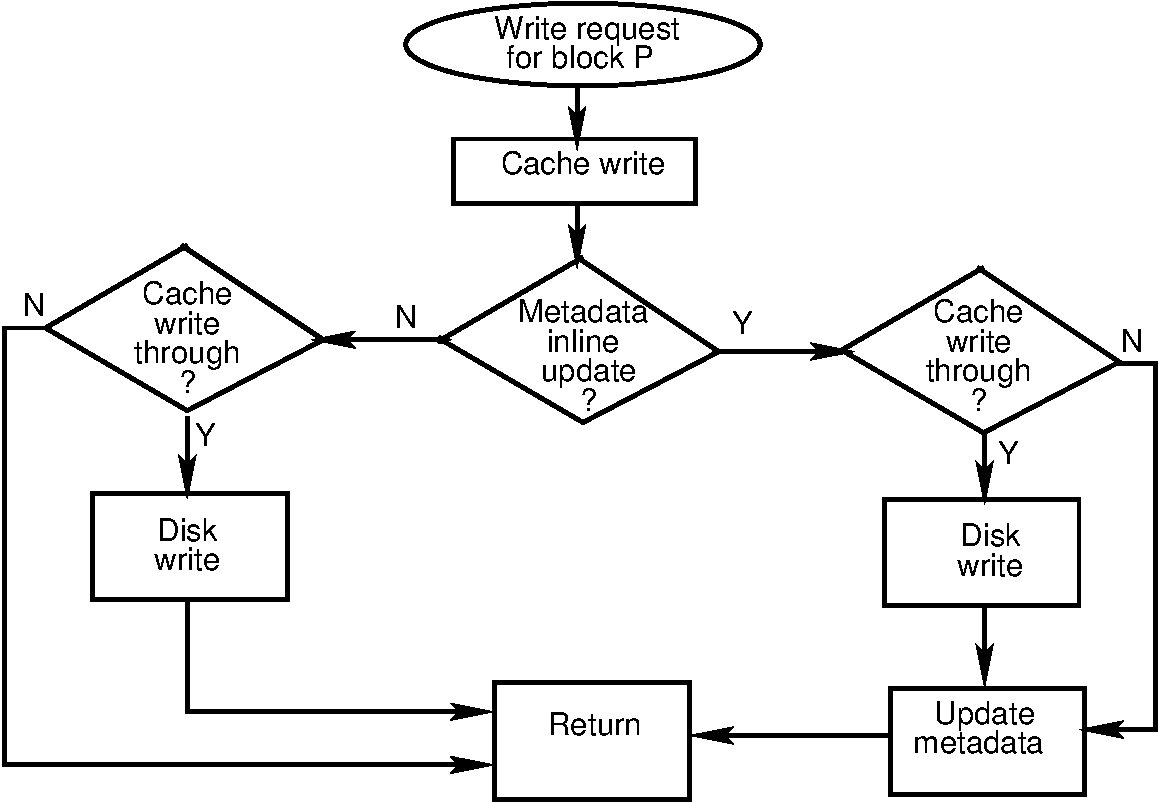
\includegraphics[scale=0.65]{confided-figures/main/dedup-working-writeflow.pdf}
    \caption{Flow path(s) for write requests in DRIVE system: \textit{Differences due to 
			cache mode (write-back, write-through) and 
			metadata update mode for writes (updated, 
			not-updated) shown.}}
    \label{fig:confided-writeflow}
%    \vspace{-0.25in}
\end{figure}

Fig.~\ref{fig:confided-writeflow} depicts the different
write paths which govern user perceived write response latency.
A write request can be executed in the following four ways, depending
upon whether the block-cache is write-through or write-back, and
whether metadata update is to be performed or not:-
(i)~Invalidate metadata, write to block-cache, return,
(ii)~Invalidate metadata, write to block-cache, write to disk, return,
(iii)~Invalidate metadata, write to block-cache, write to disk,
update metadata, return, and
(iv)~Invalidate metadata, write to block-cache, update metadata, return.

If the block-cache is a \textit{write-through} cache, the additional latency
due to metadata update (order of nanoseconds) is insignificant
relative to disk write latencies (order of milliseconds). Hence, in
case of a write-through cache, the impact of I/O deduplication overheads
on user perceived response for write requests would
be negligible. However, in case of a \textit{write-back} cache,
user perceived write-performance is dictated by the length of the
write-path till the cache, hence write-path overhead needs to be kept
as low as possible. Note that this concern does not apply to IODEDUP since
its location is downstream from the block-cache and hence needs to
handle write requests only when they are eventually flushed to disk
from block-cache. However, DRIVE is located above the
block-cache and has to perform metadata management \textit{inline} for
every write request.
%Thus, metadata update for write requests in DRIVE 
%is separated into two phases,
%with invalidation of existing metadata performed in first phase,
%and eventual update of new metadata performed in second phase (off-band).

%In the system above, metadata update performed in delayed fashion
%is said to be \textit{offband} whereas if it were performed
%in the write-path itself, it is said to be done \textit{inline}.
Alternatively, since optimizing writes is not the aim of this work, we
can still achieve correctness by only invalidating existing mappings
%(first phase above) 
for the blocks being written, \textit{without updating} the metadata.
%(second phase above).
Metadata invalidation (i.e. marking dirty) ensures that we
do not use stale metadata for redirecting subsequent read requests.
This strategy will result in lowered overhead for write requests,
but at the cost of potential performance loss due to dirty metadata 
resulting in mandatory disk fetches.
Next, we perform evaluation of DRIVE with and without metadata updates 
upon writes,
and present results to quantify its effects on performance, relative to
IODEDUP and Vanilla systems.

\subsubsection{Impact on per-request latencies due to metadata updates for writes}
\label{sec:drivechap-reqlatency}
Since DRIVE system seeks to optimize only reads and not writes, the
content of write requests is used only to invalidate existing metadata
so that stale metadata is not used for (incorrect) redirection of
subsequent read requests.
An optional task is to update the metadata
%(second phase) 
according to
the new content encountered in write requests, after having marked the
metadata dirty.
%(first phase). 
If the cache is in \textit{write-back} mode, the write path
extends
only till the block-cache, whereas if the cache is in
\textit{write-through} mode,
the write path extends all the way till disk. Hence, if metadata
update is performed \textit{inline}, it will add to the write
response latency. This metadata-update-upon-write operation
(called MeU)
is optional because it does not affect the correctness of redirection.
However, since it leaves metadata dirty, subsequent read operation may
lose optimization opportunity, hence resulting in fewer cache-hits.
Fewer cache-hits (more disk fetches) will result in
lowered throughput and on the other hand, non updation of metadata
upon write requests will incur per-write lower latencies.
We perform
study of CPU overheads under following categories:-
\begin{enumerate}
		\singlespacing
 \item Per-request read response latencies when metadata is updated 
upon writes (MeU)
\item Per-request read response latencies when metadata is not updated
upon writes (MeNU)
\item Comparison of write response latency when metadata updated (MeU)
and not (MeNU)
\end{enumerate}

\vspace{-0.1in}
\underline{Per-request read response latencies in case MeU}:
In Table~\ref{tab:readpath-list}, we list the various components involved
in the read path case-by-case, assuming that metadata update upon
writes (MeU) is being performed. In case of Vanilla, there
are only two cases for every read request:
block found in cache, i.e., \texttt{cacheR} or
block read from disk, i.e., \texttt{diskR}.
In case of DRIVE, a \texttt{diskR} can be caused due
to absent metadata, i.e., \texttt{metadatamiss} or block previously
evicted from cache, i.e., \texttt{capacitymiss}, 
whereas a \texttt{cacheR} can happen after a \texttt{metadatahit}.
In case of IODEDUP, a \texttt{cacheR} can be
due to hit in block-cache, i.e., \texttt{blockhit} or
due to hit in content-cache, i.e., \texttt{contenthit},
and a \texttt{diskR} may be inevitable in spite of a \texttt{metadatahit}, if
a \texttt{contentmiss} occurs.
The highlighted components are the overhead components, i.e. they are extra
components present in either DRIVE or IODEDUP and are not present in Vanilla
system.



\underline{Per-request read response latencies in case MeNU:}
If metadata is not updated upon write requests (MeNU) in DRIVE,
upcoming read requests
to the same block will encounter dirty metadata, i.e. \texttt{metadatamiss},
and may subsequently result in a \texttt{blockhit} or \texttt{blockmiss}.
Table~\ref{tab:readpath-list-menu} lists the components involved in the
read path in case of MeNU. Here, a \texttt{cacheR} can occur in
two ways: (i)~\texttt{metadatahit} followed by \texttt{blockhit} and
(ii)~\texttt{metadatamiss} followed by \texttt{blockhit}, and similarly
for \texttt{diskR} as well.




\vspace{1in}
\begin{landscape}
\begin{table}
\caption{Steps involved in Read-path for Vanilla, DRIVE and IODEDUP with metadata updated upon writes}
\label{tab:readpath-list}
\centering
\begin{tabular}{|l|c|c|c|c|c|c|c|c|c|} \hline
 & \multicolumn{2}{c|}{\textbf{Vanilla}} & \multicolumn{3}{c|}{\textbf{DRIVE (with MeU)}} & \multicolumn{4}{c|}{\textbf{IODEDUP (with MeU)}}  \\ \cline{2-10}
 & & & \texttt{cacheR} & \multicolumn{2}{c|}{\texttt{diskR}} & \multicolumn{2}{c|}{\texttt{cacheR}} & \multicolumn{2}{c|}{\texttt{diskR}} \\ \cline{4-10}
 & & & \texttt{block} & \texttt{metadata} & \texttt{block} & \texttt{block} & \texttt{content} & \texttt{metadata} & \texttt{content} \\
\textbf{Step} & \texttt{cacheR} & \texttt{diskR} & \texttt{hit} & \texttt{miss} & \texttt{miss} & \texttt{hit} & \texttt{hit} & \texttt{miss} & \texttt{miss} \\ \hline
\rowcolor{Gray} \textit{Metadata lookup} & & & \ding{51} & \ding{51} & \ding{51} & & \ding{51} &\ding{51} & \ding{51} \\
\textit{Block-cache lookup} & \ding{51} & \ding{51} & \ding{51} & \ding{51} & \ding{51} & \ding{51} & \ding{51} & \ding{51} & \ding{51} \\
\rowcolor{Gray} \textit{Content-cache lookup} & & & & & & & \ding{51} & & \ding{51} \\
\textit{Disk read} & & \ding{51} & & \ding{51} & \ding{51} & & & \ding{51} & \ding{51}  \\
\textit{Block-cache update} & & \ding{51} & & \ding{51} & \ding{51} & & \ding{51} & \ding{51} & \ding{51} \\
\rowcolor{Gray} \textit{Metadata update} & & & & \ding{51} & & & & \ding{51} & \\
\rowcolor{Gray} \textit{Content-cache update} & & & & & & & & \ding{51} & \ding{51} \\ \hline \hline
\textit{Total read latency} & 83ns &$\sim$13.7ms & 183ns & $\sim$13.7ms & $\sim$13.7ms & 83ns & 383ns & $\sim$13.7ms & $\sim$13.7ms  \\ \hline
\end{tabular}
%\vspace{-0.15in}
\end{table}

\begin{table}
\caption{Components in Read-path latency for Vanilla, DRIVE and IODEDUP with metadata NOT updated upon writes}
\label{tab:readpath-list-menu}
\centering
\begin{tabular}{|l|c|c|c|c|c|c|c|c|c|c|c|c|c|c|c|c|} \hline
 & \multicolumn{2}{c|}{\textbf{Vanilla}} & \multicolumn{4}{c|}{\textbf{DRIVE (with MeNU)}} & \multicolumn{4}{c|}{\textbf{IODEDUP (with MeNU)}}  \\ \cline{2-11}
 & & & \multicolumn{2}{c|}{\texttt{cacheR}} & \multicolumn{2}{c|}{\texttt{diskR}} & \multicolumn{2}{c|}{\texttt{cacheR}} & \multicolumn{2}{c|}{\texttt{diskR}} \\ \cline{4-11}
 & & &\texttt{metadata} & \texttt{metadata} & \texttt{metadata} & \texttt{metadata} &  & &  &  \\
 & & &\texttt{hit}      & \texttt{miss} & \texttt{miss} & \texttt{hit} &  & &  &  \\
 & & &\texttt{block}    & \texttt{block} & \texttt{block} & \texttt{block} & \texttt{block} & \texttt{content} & \texttt{metadata} & \texttt{content} \\
\textbf{Component} & \texttt{cacheR} & \texttt{diskR} & \texttt{hit} & \texttt{hit} & \texttt{miss} & \texttt{miss} & \texttt{hit} & \texttt{hit} & \texttt{miss} & \texttt{miss} \\ \hline
\rowcolor{Gray} \textit{Metadata lookup} & & & \ding{51} & \ding{51} & \ding{51} & \ding{51} & & \ding{51} &\ding{51} & \ding{51} \\
\textit{Block-cache lookup} & \ding{51} & \ding{51} & \ding{51} & \ding{51} & \ding{51} & \ding{51} & \ding{51} & \ding{51} & \ding{51} & \ding{51} \\
\rowcolor{Gray} \textit{Content-cache lookup} & & & & & & & & \ding{51} & & \ding{51} \\
\textit{Disk read} & & \ding{51} & & & \ding{51} & \ding{51} & & & \ding{51} & \ding{51}  \\
\textit{Block-cache update} & & \ding{51} & &  & \ding{51} & \ding{51} & & \ding{51} & \ding{51} & \ding{51} \\
\rowcolor{Gray} \textit{Metadata update} & & & & \ding{51} & \ding{51} & & & & \ding{51} & \\
\rowcolor{Gray} \textit{Content-cache update} & & & & & & & & & \ding{51} & \ding{51} \\ \hline \hline
\textit{Total latency per request} & 83ns & $\sim$13.7ms & 183ns & 33$\mu$s & $\sim$13.7ms & $\sim$13.7ms & 83ns & 383ns & $\sim$13.7ms & $\sim$13.7ms  \\ \hline
\end{tabular}
%\vspace{-0.15in}
\end{table}
\end{landscape}

%\begin{table*}
%\caption{Components in Write-path latency for Vanilla, DRIVE and IODEDUP with MeU and MeNU}
%\label{tab:writepath-list}
%\centering
%\begin{tabular}{|l|c|c|c|c|c|c|c|c|c|c|} \hline
% & \multicolumn{2}{c|}{\textbf{Vanilla}} & \multicolumn{4}{c|}{\textbf{DRIVE}} & \multicolumn{4}{c|}{\textbf{IODEDUP}}  \\ \cline{2-11}
% & & & \multicolumn{2}{c|}{\texttt{Write-through}} & \multicolumn{2}{c|}{\texttt{Write-back}} & \multicolumn{2}{c|}{\texttt{Write-through}} & \multicolumn{2}{c|}{\texttt{Write-back}} \\ \cline{4-11}
%\textbf{Component} & \texttt{Write-through} & \texttt{Write-back} & \texttt{MeU} & \texttt{MeNU} & \texttt{MeU} & \texttt{MeNU} & \texttt{MeU} & \texttt{MeNU} & \texttt{MeU} & \texttt{MeNU} \\ \hline
%\rowcolor{Gray} \textit{Metadata invalidate} & & & \ding{51} & \ding{51} & \ding{51} & \ding{51} & & &  & \\
%\textit{Block-cache update} & \ding{51} & \ding{51} & \ding{51} & \ding{51} & \ding{51} & \ding{51} & \ding{51} & \ding{51} & \ding{51} & \ding{51} \\ 
%\textit{Disk write} & \ding{51} & & \ding{51} & \ding{51} & & & \ding{51} & \ding{51} &  & \\ 
%\rowcolor{Gray} \textit{Metadata update} & & & \ding{51} & & \ding{51} & & & &  & \\ \hline \hline
%%\textit{Content-cache update} & & & & & & & \ding{51} & \ding{51} & \ding{51} & \ding{51} \\ \hline
%\textit{Total latency per request}    & $\sim$15ms & 100ns& $\sim$15ms  & $\sim$15ms & $\sim$33.33us& 200ns & $\sim$15ms & $\sim$15ms& 100ns & 100ns \\ \hline
%\end{tabular}
%%\vspace{-0.15in}
%\end{table*}

\underline{Comparison of write latency when MeU versus MeNU:}
Metadata update during write requests
will add to write response latency, whereas only performing metadata
invalidation not only ensures that dirty metadata is not used for
redirection, but also keeps the write-response timings low, especially
in case of a write-back cache.

Possible write paths that contribute to write response latency for Vanilla,
DRIVE and IODEDUP are listed in Table~\ref{tab:writepath-list}.
As shown, when the cache is in write-through mode, metadata update latency
makes little difference to the write response latency since disk
write latency is the dominant component in this case.
However, when the block-cache is in write-back mode, writes are only
written to cache, so metadata update contributes comparable overhead to the
write path latency. So, we explore two options of (i) updating metadata,
and (ii) not updating metadata, and the corresponding hourly throughput is
reported in Table~\ref{tab:writepath-list}.
Note that IODEDUP has no overhead in the write path when the block-cache is in
write-back mode. This is because, as described earlier, IODEDUP is positioned
downstream from the block-cache and encounters write requests only when
they are flushed from (not when they are written to) cache in case of a
write-back cache.

Depending upon whether the block-cache is
in write-through or write-back mode, and whether the metadata is updated
(MeU) or not-updated (MeNU) upon write request, the read and
write response latencies can vary. Moreover, the number of cache-hits in
each case is also influenced by the same reasons. Next,
we present comparative evaluation of the three systems using various metrics
like  cache-hit ratios, number of disk reads averted, average read response
latency and throughput.

\begin{table}[t]
\caption{Write-path latency for Vanilla, DRIVE and IODEDUP with MeU and MeNU}
\label{tab:writepath-list}
\centering
\begin{tabular}{|l|c|c|c|c|} \hline
\textbf{Write-through} & \textbf{System} & \textbf{Metadata} & \textbf{Latency} & \textbf{Throughput} \\
\textbf{or Write-back} & & \textbf{Update?}  & \textbf{per request} & \textbf{(million per hour)} \\ \hline
Write-through & Vanilla & - & $\sim$15ms & 0.216 \\
Write-through & DRIVE & MeU & $\sim$15ms & 0.216 \\
Write-through & DRIVE & MeNU & $\sim$15ms & 0.216 \\
Write-through & IODEDUP & - & $\sim$15ms & 0.216 \\ \hline
Write-back & Vanilla & - & 100ns & 36000 \\
Write-back & DRIVE & MeU & $\sim$33.33$\mu$s & 108 \\
Write-back & DRIVE & MeNU & 200ns & 18000 \\
Write-back & IODEDUP & - & 100ns & 36000 \\ \hline
\end{tabular}
%\vspace{-0.15in}
\end{table}

%\subsection{Impact on cache effectiveness due to metadata updates for writes}
%In Section \ref{sec:drivechap-reqlatency} above, we studied the 
%impact of metadata updates for writes on per-request latency for both
%read and write requests. Now, we explore the variation in cache
%deduplication effectiveness due to MeU versus MeNU.
%
%details pending.

\subsection{Cost-benefit analysis of metadata space usage in DRIVE versus \\IODEDUP}
Both the DRIVE and IODEDUP systems maintain metadata stores, which 
basically identify similarity across blocks using content fingerprints.
The difference between the two systems, though, is the placement of
the metadata store\textemdash{}in IODEDUP, the metadata store is present downstream
of the host-cache, whereas DRIVE system has it upstream of the cache.
Metadata space is basically occupying precious space~\cite{idedup} otherwise 
available for caching, hence, we need to analyze the cost
and benefit of using a metadata store. 

In the previous section, we demonstrated that DRIVE system is able
to achieve better performance than Vanilla system, using a metadata store
metadata store and simple hint-based I/O redirection. Thus, the benefit
of the metadata store is justified in that case.
The IODEDUP system also uses a metadata store, and performs I/O
deduplication, so here we perform a comparison to see which one
of the two systems (DRIVE or IODEDUP) is able to make better use
of the precious cache space. 

Both the IODEDUP and DRIVE systems build metadata at runtime, i.e.,
intercept requests and compare content fingerprints to determine
whether content is new or duplicate\textemdash{}in both cases, metadata 
is updated accordingly. If these systems are deployed on 
production systems that are used long-term, the metadata store
will keep growing, unless it is managed as a fixed-size metadata cache.
Note that, pruning of metadata in this manner may result in some
lost deduplication opportunities, but the rest of the metadata
can still yield better performance than the Vanilla system.

For the purpose of this thesis, the aspect of metadata space 
management is not within thesis scope (it is future work), and
metadata space management has not been discussed in 
IODEDUP paper~\cite{iodedup} either.
So, for comparison between IODEDUP and DRIVE system using the 
available traces~\cite{iodedup-online}, we assume
that metadata storage space is sufficient to store all metadata
for these traces.
Observe that, this is
the best case scenario for both DRIVE and IODEDUP systems,
since there will no lost deduplication opportunities here.
Moreover, this space usage will be approximately equal (say, $x$ MB)
in both DRIVE and IODEDUP systems, so here we compare the cost and 
benefit of using $x$ MB space as a metadata store in both systems.

\paragraph{Cost of metadata store:} 
As mentioned above, the positioning of the metadata store is
different (downstream versus upstream) in IODEDUP and DRIVE systems.
Despite this, both systems have to track every ``new'' content 
and update metadata accordingly\textemdash{}and hence, space occupied
by metadata in both systems will be equal for any given workload/trace.
Thus, the ``cost'' of metadata store is equivalent in both systems.
However, the benefit of metadata store is different in both the
systems, and we demonstrate it next.

\paragraph{Benefits of metadata store:}
Metadata can be said to be beneficial when it results in a cache 
hit (i.e., disk fetch is averted) which would not have been otherwise possible.
For example, if blocks A and B are duplicates of each other, and both
are in cache, then a cache hit for either of them can not be considered
as a ``benefit'' of metadata. On the other hand, if only block A is present in 
cache, and a request for block B could be satisfied due to deduplication,
that is a benefit of having relevant metadata. We define the former case
as a \texttt{self-hit} and the latter as a \texttt{dedup-hit}, and claim
that only the number of \texttt{dedup-hits} determines the benefit of 
gathering similarity-based metadata. %in both IODEDUP and DRIVE systems.

\underline{Number of read requests encountering metadata hits:}
In DRIVE, every block-cache lookup (and disk fetch, if required) happens
after \texttt{metadatahit} or \texttt{metadatamiss}. However, 
in case of IODEDUP, only requests that encounter \texttt{blockmiss}
get looked up into metadata (refer the discussion in previous section for details).
This is because DRIVE metadata store is upstream of the block-cache,
whereas IODEDUP metadata store is downstream. This implies that,
the total number of metadata hits in DRIVE will be potentially 
higher than in IODEDUP, and this is reflected in Table~\ref{tab:num-metadata-hits}.
It can be seen that for each trace\textemdash{}\textit{webvm}, \textit{homes}, 
\textit{mail}\textemdash{}the
total number of metadata hits in DRIVE system is higher than in IODEDUP.

\begin{table}[t]
	\caption{Number of metadata hits encountered for read requests}
	\label{tab:num-metadata-hits}
	\centering
	\begin{tabular}{|c|c|c|c|} \hline
		\textbf{Trace} & \textbf{Scheme} & \textbf{Num. of read} & \textbf{Num. of} \\
			  \textbf{name} & \textbf{name} & \textbf{requests} & \textbf{metadata hits} \\ \hline
		\textit{homes} & IODEDUP & 4,052,176 & 647,012 \\ \hline
	   	\textit{homes} & DRIVE & 4,052,176 & 695,747 \\ \hline
		\textit{mail} & IODEDUP & 2,375,409 & 382,119 \\ \hline
		\textit{mail} & DRIVE & 2,375,409 & 625,938 \\ \hline
	    \textit{webvm} & IODEDUP & 3,116,456 & 2,223,457 \\ \hline
		\textit{webvm} & DRIVE & 3,116,456 & 2,800,411 \\ \hline
	\end{tabular}
	%\vspace{-0.15in}
\end{table}



\underline{Classification of metadata hits:}
As mentioned earlier, a \texttt{metadatahit} does not guarantee that
a cache-hit will occur\textemdash{}that is, \texttt{metadatahit} can result 
in either a cache hit or a miss. And each of these hits/misses
can further be classified into (i)~\texttt{self-hit}, 
(ii)~\texttt{self-miss}, 
(iii)~\texttt{dedup-hit}, and
(iv)~\texttt{dedup-miss}. Basically the prefix ``self'' indicates
that the request was for the same block itself, whereas ``dedup''
indicates that the request was for another block and the metadata
store could successfully identify it as a duplicate.
In Fig.~\ref{fig:metadata-conversions}, we present a classification
of the total number of metadata hits into one of these four
classes, for each trace under both IODEDUP and DRIVE systems.

\begin{figure}
    \centering
    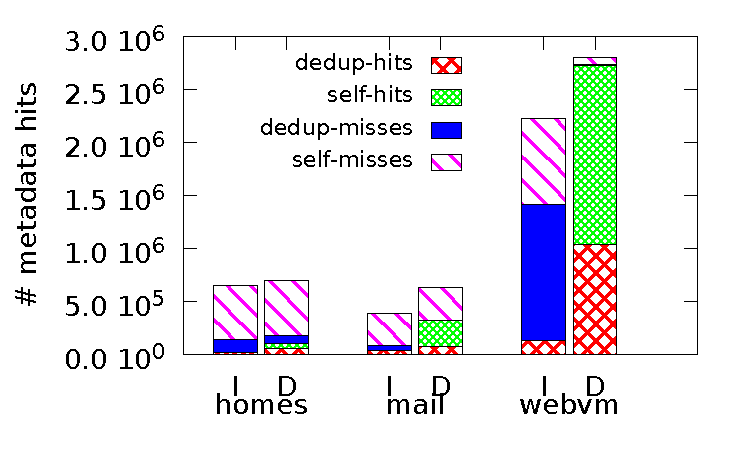
\includegraphics[scale=0.85]{confided-figures/metadata-conversions/reads-writes/metadataconversions-reads-n-writes.pdf}
    \caption{Classification of metadata hits in IODEDUP(I) Vs DRIVE(D) for the \textit{homes}, \textit{mail} and \textit{webvm} traces.}
    \label{fig:metadata-conversions}
\end{figure}

\begin{table}[t]
	\caption{Capturing \textit{metadata benefit ratio}}
	\label{tab:metadata-benefits}
	\centering
	\begin{tabular}{|c|c|c|c|c|} \hline
		\textbf{Trace} & \textbf{Scheme} & \textbf{Num. of} & \textbf{Num. of} & \textbf{Benefit} \\
			  \textbf{name} & \textbf{name} & \textbf{metadata hits} & \textbf{dedup-hits} & \textbf{ratio(\%)} \\ \hline
		\textit{homes} & IODEDUP & 647,012 & 14,041 & 2.17 \\ \hline
	   	\textit{homes} & DRIVE & 695,747 & 51,090 & 7.34 \\ \hline
		\textit{mail} & IODEDUP & 382,119 & 31,934 & 8.36 \\ \hline
		\textit{mail} & DRIVE & 625,938 & 74,673 & 11.93 \\ \hline
	    \textit{webvm} & IODEDUP & 2,223,457 & 127,156 & 5.72 \\ \hline
		\textit{webvm} & DRIVE & 2,800,411 & 1,033,328 & 36.90 \\ \hline
	\end{tabular}
	%\vspace{-0.15in}
\end{table}

From Fig.~\ref{fig:metadata-conversions}, we can see that the total number
of metadata hits is greater in DRIVE system than IODEDUP system, for all traces.
Moreover, in case of \textit{webvm} trace, most of metadata hits in IODEDUP
system result in \texttt{dedup-misses} or \texttt{self-misses}, while
DRIVE is able to convert most of its metadata hits into \texttt{dedup-hits}
and \texttt{self-hits}. This leads to the huge performance improvement
by DRIVE system for \textit{webvm} trace, as compared to IODEDUP system.

\underline{Differentiating self-hits and dedup-hits:}
The above Fig.~\ref{fig:metadata-conversions} shows that for \textit{webvm}
trace, DRIVE has higher number of \texttt{dedup-hits} \textit{plus} \texttt{self-hits}
than IODEDUP. However, as explained earlier, only the number of \texttt{dedup-hits}
should be considered as a ``benefit'' of using the metadata store. 
Hence, if we want to capture metadata benefits using a single number, it would be
the ratio of number of \texttt{dedup-hits} to number of \texttt{metadatahits}.
Table~\ref{tab:metadata-benefits} presents this ratio for each of the traces, 
and we can see that DRIVE system has a higher metadata benefit ratio than IODEDUP,
for all three workloads considered.
Especially, for \textit{webvm} trace which was found to be an ideal candidate to
benefit from I/O deduplication, the DRIVE system has more than 6$\times$ higher
metadata benefit ratio than IODEDUP system. 
\\
\\
\underline{Implications of metadata benefit ratio on metadata store size:}
In Table~\ref{tab:metadata-benefits}, we see that when the metadata store
size is equal, the benefits achieved by DRIVE system is higher than by IODEDUP
system. This effectively implies the following:-
\begin{enumerate}
\item For IODEDUP to achieve similar benefits as DRIVE, it needs 
a much larger metadata store and/or content-cache, whereas
\item For DRIVE to attain the same performance as IODEDUP, it may only need
a relatively smaller metadata store.
\end{enumerate}

Based on the analysis presented in this section, we have proven that
the DRIVE system achieves much better I/O deduplication performance
than IODEDUP system, for the same size of metadata store. Specifically,
the DRIVE system achieves lower read response latencies, and higher
metadata benefit ratio than the IODEDUP system.
